%%%%%%%%%%%%%%%%%%%%%%%%%%%%%%%%%%%%%%%%%%%%%%%%%%%%%%%%%%%%%%%%%%%%%%
% writeLaTeX Example: A quick guide to LaTeX
%
% Source: Dave Richeson (divisbyzero.com), Dickinson College
% 
% A one-size-fits-all LaTeX cheat sheet. Kept to two pages, so it 
% can be printed (double-sided) on one piece of paper
% 
% Feel free to distribute this example, but please keep the referral
% to divisbyzero.com
% 
%%%%%%%%%%%%%%%%%%%%%%%%%%%%%%%%%%%%%%%%%%%%%%%%%%%%%%%%%%%%%%%%%%%%%%
% How to use writeLaTeX: 
%
% You edit the source code here on the left, and the preview on the
% right shows you the result within a few seconds.
%
% Bookmark this page and share the URL with your co-authors. They can
% edit at the same time!
%
% You can upload figures, bibliographies, custom classes and
% styles using the files menu.
%
% If you're new to LaTeX, the wikibook is a great place to start:
% http://en.wikibooks.org/wiki/LaTeX
%
%%%%%%%%%%%%%%%%%%%%%%%%%%%%%%%%%%%%%%%%%%%%%%%%%%%%%%%%%%%%%%%%%%%%%%

\documentclass[a4paper]{article}
\usepackage{amssymb,amsmath,amsthm,amsfonts}
\usepackage{multicol,multirow}
\usepackage{calc}
\usepackage{ifthen}
\usepackage[landscape]{geometry}
\usepackage[colorlinks=true,citecolor=blue,linkcolor=blue]{hyperref}
\usepackage{graphicx}


\ifthenelse{\lengthtest { \paperwidth = 11in}}
    { \geometry{top=.5in,left=.5in,right=.5in,bottom=.5in} }
	{\ifthenelse{ \lengthtest{ \paperwidth = 297mm}}
		{\geometry{top=1cm,left=1cm,right=1cm,bottom=1cm} }
		{\geometry{top=1cm,left=1cm,right=1cm,bottom=1cm} }
	}

\pagestyle{empty}
\makeatletter
\renewcommand{\section}{\@startsection{section}{1}{0mm}%
                                {-1ex plus -.5ex minus -.2ex}%
                                {0.5ex plus .2ex}%x
                                {\normalfont\large\bfseries}}
\renewcommand{\subsection}{\@startsection{subsection}{2}{0mm}%
                                {-1explus -.5ex minus -.2ex}%
                                {0.5ex plus .2ex}%
                                {\normalfont\normalsize\bfseries}}
\renewcommand{\subsubsection}{\@startsection{subsubsection}{3}{0mm}%
                                {-1ex plus -.5ex minus -.2ex}%
                                {1ex plus .2ex}%
                                {\normalfont\small\bfseries}}
\makeatother
\setcounter{secnumdepth}{0}
\setlength{\parindent}{0pt}
\setlength{\parskip}{0pt plus 0.5ex}
% -----------------------------------------------------------------------

\title{MTE321 Formulas}

\begin{document}

\raggedright
\footnotesize

\begin{center}
     \Large{\textbf{MTE321 Formulas}} \\
\end{center}
\begin{multicols}{3}
\setlength{\premulticols}{1pt}
\setlength{\postmulticols}{1pt}
\setlength{\multicolsep}{1pt}
\setlength{\columnsep}{2pt}


\section{Stresses}
\subsection{Deformation Elongation}
\begin{align*}
    \delta = \frac{FL}{EA}\\
    \delta = \frac{\sigma L}{E}
\end{align*}


\subsection{Torsional Forumals}
\subsubsection{Stress}
R is the radial distance
\begin{align*}
    \tau = \frac{Tr}{J}\\
    Z_p = \frac{J}{c}\\
    \tau_{max} = \frac{T}{Z_p}
\end{align*}

\subsubsection{Deformation}
$\theta$ is the angle of twist across L\\
For non-circular shafts K is section polar second moment of area and Q the section polar modulus
\begin{align*}
	T = \frac{P}{\omega} \hspace{2mm} T_{lb\cdot in}=63000\frac{P}{\omega}\\
    \theta = \frac{TL}{GJ}\\
    \textit{Non-Circular }\tau = \frac{T}{Q}\\
    \textit{Non-Circular }\theta = \frac{TL}{GK}
\end{align*}
\subsubsection{Thin-Walled Closed Tubes}
A = median area boundary, U is length of median boundary
\begin{align*}
	K = \frac{4A^2t}{U}\\
	Q = 2tA\\
\end{align*}
\subsection{Shear Stress}
V section shear force, Q is the first moment area, and t is the section thickness
\begin{align*}
	\tau_{(y)} = \frac{VQ}{It}\\
	\textit{Rectangular Beam }\tau_{max} = \frac{3V}{2A}\\
	\textit{Solid Round Beam }\tau_{max} = \frac{4V}{3A}\\
	\textit{Hollow Round Beam }\tau_{max} = \frac{2V}{A}
\end{align*}

\subsubsection{Beam Bending}
M is the moment at the section, y is the distance from the neutral axis
\begin{align*}
    \sigma_{y} = -\frac{My}{I}
\end{align*}

\section{Stress Concentrations}

\subsection{Stress Concentration Factor}
K\textsubscript{t} is material and loading dependent, values greater than 3 are a waste
\begin{align*}
    \sigma_{max} = K_t\sigma_{nom}
\end{align*}
\subsubsection{Curved Beam Bending}
R = $\frac{A}{ASF}$\\
r = distance to required stress location\\
r\textsubscript{c}= centroid distance\\
A = cross-sectional area\\
\begin{align*}
	\sigma_{(r)} = \frac{M(\theta)(R-r)}{Ar(r_c-R)}
\end{align*}
\subsection{Thermal Strain}
\begin{align*}
	\epsilon_x^m=-\alpha\Delta T
\end{align*}
\subsection{Principle Stresses}
\begin{align*}
	tan2\theta_\sigma = \frac{2\tau_{xy}}{\sigma_x-\sigma_y}\\
	\sigma_{1,2} = \frac{\sigma_x + \sigma_y}{2} \pm \sqrt{\left(\frac{\sigma_x-\sigma_y}{2}\right)^2 + \tau^2_{xy}}\\
	\textit{Max }\sigma_{norm} = \frac{1}{2}(\sigma_x + \sigma_y) + \sqrt{\left[\frac{1}{2}\sigma_x-\sigma_y\right]^2 + \tau_{xy}^2}\\
	\textit{Min }\sigma_{norm} = \frac{1}{2}(\sigma_x - \sigma_y) - \sqrt{\left[\frac{1}{2}\sigma_x-\sigma_y\right]^2 + \tau_{xy}^2}\\
\end{align*}
\section{Design Factors}
\subsection{A\textsubscript{95} Equivalence}
\begin{align*}
\textit{Equivalent Diameter: }D_e=0.370D\\
\textit{General: }0.766D_e^2\\
\end{align*}
\section{Design: Dynamic Loads}
\subsection{Loading}
\begin{align*}
	\sigma_m =\textit{mean stress  } = \frac{\sigma_{max} + \sigma_{min}}{2} \\
	\sigma_a = \textit{stress amplitude  } = \frac{\sigma_{max} - \sigma_{min}}{2}\\
	R = \textit{stress ratio} = \frac{\sigma_{min}}{\sigma_{max}}\\
	A = \textit{stress ratio  } = \frac{\sigma_a}{\sigma_m}\\
	\textit{Loading Cycle: preriod between peaks }
\end{align*}
\subsection{Stress}
\subsubsection{Periodic}
Fluctuating $\sigma_m \neq 0$ , R = -1\\
Pulsating $\sigma_m = 0$, R =1\\
\subsubsection{Endurance Limit}
s\textsubscript{a} =Stress Amplitude Level\\
N: number of cycles to failure\\
s\textsubscript{n} = fatigue limit\\
Assume s\textsubscript{n} = 0.5s\textsubscript{u} if no data\\
\begin{align*}
s_a = s_nN^b\\
s^`_n = C_mC_{st}C_RC_Ss_n\\
\end{align*}
s\textsubscript{n} from table appendix 3\\
C\textsubscript{m} material flaws\\
C\textsubscript{R} Reliability Factor\\
C\textsubscript{s} = size factor (5-12,5-4 circular),(5-13 for other)\\
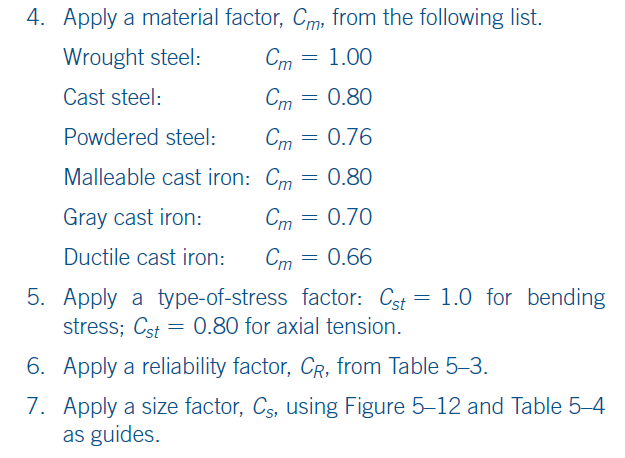
\includegraphics[scale=0.5]{ActualEnduranceLimit.png}
\subsection{Goodman Method}
\subsubsection{Dynamic Loads Ductile}
\begin{align*}
(\sigma_m < 0)\\
\textit{Von Mises: } N_1 = \frac{s^`_n}{K_t\sigma^`_a}\\
\textit{Tresca: } N_1 = \frac{s^`_n}{K_t\sigma^`_a}\\
\end{align*}
\subsubsection{Dynamic Loads Tensile}
\begin{align*}
(\sigma_m > 0)\\
\textit{Von Mises: } \frac{K_t\sigma^`_a}{s^`n} + \frac{\sigma^`_m}{s_u} = \frac{1}{N_1}\\
\textit{Tresca: } \frac{2K_t}{s^`_n}(\tau_a)_{max} + \frac{4}{3s_u}(\tau_m)_{max} = \frac{1}{N_1}\\
\end{align*}
\subsubsection{Dynamic Yield Test}
\begin{align*}
\textit{for low }\sigma_a\textit{ high }\sigma_m\\
\textit{Von Mises: } \frac{K_t\sigma^`_a}{s_{y}} + \frac{K_t\sigma^`_m}{s_y} = \frac{1}{N_2}\\
\textit{Tresca: } \frac{2K_t}{s_{sy}}(\tau_a)_{max} + \frac{2K_t}{S_{sy}}(\tau_m)_{max} = \frac{1}{N_2}
\end{align*}
Effective safety factor is < of N\textsubscript{1} and N\textsubscript{2}
\section{Gears}
Table 8-1\\
\subsection{Pitch Line Speed}
\begin{align*}
V_T = \frac{\pi D\cdot n_p}{12}
\end{align*}
\section{Gears}
\subsection{Spur Gears}
\begin{align*}
\textit{Speed of Gears: } \frac{n_p}{n_G}=\frac{N_G}{N_P}\\
\textit{Common Speed: } v_T = R_1\omega_1 = R_2\omega_2 \\
\textit{Tangental Acceleration: }a_T = R_1\alpha_1 = R_2\alpha_2\\
\textit{Velocity Ratio: } VR = \frac{R_G}{R_P} >= 1\\
\textit{Circular Pitch: } p = \frac{\pi D}{N}\\
\textit{Contact Ratio: }\\
\end{align*}
\subsection{Helical Gears}
\begin{align*}
\textit{Transverse Pitch: } \frac{\pi}{P_d}\\
\textit{Normal Circular: }p_n = p+ \cos\psi \\
\textit{Axial Pitch: }p_x = \frac{p_t}{\tan\psi}\\
\end{align*}
\end{multicols}
\end{document}
